\chapter{Języki, automaty i obliczenia}

Materiały teoretyczne z tego przedmiotu zostały opracowane na podstawie \href{https://www.mimuw.edu.pl/~szymtor/jao/skrypt.pdf}{skryptu Szymona Toruńczyka}.

\section*{Podstawa programowa}
\begin{enumerate}
    \item \textbf{Języki regularne}, wyrażenia regularne, automaty skończone.
    \item \textbf{Języki bezkontekstowe}, gramatyki bezkontekstowe, automaty ze stosem.
    \item \textbf{Lematy o pompowaniu} dla języków regularnych i bezkontekstowych.
    \item \textbf{Języki obliczalne} i częściowo obliczalne. Problem stopu oraz metoda przekątniowa.
    \item \textbf{Klasy P, NP} oraz NP-zupełność.
\end{enumerate}

% Filip
\section{Języki regularne}

\textbf{Automat niedeterministyczny (NFA)} to krotka $\langle A, Q, I, F, \delta \rangle$, gdzie:

\begin{itemize}
    \item $A$ to alfabet, czyli skończony zbiór symboli zwanych dalej \textit{literami},
    \item $Q$ to skończony zbiór stanów,
    \item $I \subseteq Q$ to zbiór stanów początkowych,
    \item $F \subseteq Q$ to zbiór stanów akceptujących,
    \item $\delta \subseteq Q \times A \times Q$ to relacja przejścia.
\end{itemize}

\textbf{Automat deterministyczny (DFA)} to prawie taka sama krotka $\langle A, Q, I, F, \delta \rangle$ jak powyżej, ale z tą różnicą, że $\delta$ to funkcja typu $Q \times A \to Q$, a nie tylko relacja.

\textbf{Automat z $\epsilon$-przejściami} to automat dopuszczający przejścia postaci $(p, \epsilon, q)$, gdzie $\epsilon$ to słowo puste.

Terminologia:
\begin{itemize}
    \item \textit{tranzycja (przejście)} -- trójka $(p, a, q) \in \delta$, również oznaczana jako $p \xrightarrow{a} q$,
    \item \textit{bieg} -- ciąg tranzycji $q_0 \xrightarrow{a_1} q_1 \xrightarrow{a_2} q_2 \xrightarrow{a_3} \ldots \xrightarrow{a_n} q_n$, gdzie $q_0 \in I$ i który można interpretować jako ścieżkę w grafie automatu,
    \item \textit{bieg akceptujący} -- bieg, który kończy w stanie akceptującym,
    \item \textit{bieg po słowie $w$} -- bieg $q_0 \xrightarrow{a_1} q_1 \xrightarrow{a_2} q_2 \xrightarrow{a_3} \ldots \xrightarrow{a_n} q_n$ taki, że $a_1 a_2 a_3 \ldots a_n = w$.
    \item automat $\mathcal{A}$ \textit{akceptuje} słowo $w \in A^*$, jeżeli istnieje bieg akceptujący po tym słowie,
    \item automat $\mathcal{A}$ \textit{rozpoznaje} język $L$, jeśli $w \in L \wtw \mathcal{A}$ akceptuje $w$ i oznaczamy to jako $L = \mathcal{L}(A)$.
\end{itemize}

\textbf{Wyrażenie regularne} to wyrażenie zbudowane rekurencyjnie, które reprezentuje pewien język. Tak samo jak dla automatów, dla wyrażenia regularnego $A$ reprezentującego język $L$ piszemy, że $L = \mathcal{L}(A)$. Można je budować przy pomocy następujących reguł:
\begin{itemize}
    \item $\emptyset$ jest wyrażeniem regularnym reprezentującym język pusty,
    \item $a$ jest wyrażeniem regularnym reprezentującym język $A = \{ a \}$,
    \item dla wyrażeń $A, B$: $A + B$ reprezentuje język $\mathcal{L}(A) \cup \mathcal{L}(B)$,
    \item dla wyrażeń $A, B$: $A \cdot B$ (lub po prostu $AB$) reprezentuje język $K \cdot L = \{ v \cdot w \mid v \in K, w \in L \}$, gdzie $K = \mathcal{L}(A), L = \mathcal{L}(B)$,
    \item dla wyrażenia $A$: $A^*$ reprezentuje język $\{ w_1 \cdot w_2 \cdot \ldots \cdot w_n \mid w_1, w_2, \ldots, w_n \in \mathcal{L}(A), n \in \mathbb{N} \}$.
\end{itemize}

Prawdziwy jest następujący \textbf{lemat o równoważności automatów i wyrażeń regularnych}: niech $L \subseteq A^*$. Następujące warunki są równoważne:
\begin{itemize}
    \item język $L$ jest reprezentowany przez pewne wyrażenie regularne,
    \item język $L$ jest rozpoznawany przez pewien automat niedeterministyczny,
    \item język $L$ jest rozpoznawany przez pewien automat deterministyczny,
    \item język $L$ jest rozpoznawany przez pewien automat (nie)deterministyczny z $\epsilon$-przejściami.
\end{itemize}

Języki regularne są zamknięte na:
\begin{itemize}
    \item \textbf{sumę} -- dla języków regularnych $K$ i $L$, język 
    $K \cup L$ jest regularny.
    \item \textbf{konkatenację} -- dla języków regularnych $K$ i $L$, język $K \cdot L = \{ w_K \cdot w_L : w_K \in K, w_L \in L \}$ jest regularny.
    \item \textbf{gwiazdkę Kleene'ego} -- dla języka regularnego $L$,
    język $L^* = \{ w_1 \cdot w_2 \cdot \ldots \cdot w_n : w_1, w_2, \ldots, w_n \in L,
    n \in \mathbb{N} \}$
    jest regularny.
    \item \textbf{przecięcie} -- dla języków regularnych $K$ i $L$, język $K \cap L$ jest regularny.
    \item \textbf{dopełnienie} -- dla języków regularnych $K$ i $L$, język $K - L$ jest regularny.
    \item \textbf{odwrócenie języka} -- Dla języka regularnego $L$, język $L^R = \{w^R \mid w \in L\}$ jest regularny.
\end{itemize}

\subsection{Minimalizacja automatów}
Ponieważ wiele automatów może rozpoznawać ten sam język regularny, możemy rozważać \textbf{problem minimalizacji} -- jaka jest najmniejsza liczba stanów, jaką musi posiadać automat, żeby rozpoznawał dany język? Rozważany automat będzie automatem \textit{deterministycznym} i będzie nazywany \textit{automatem syntaktycznym}. Do znalezienia takiego automatu przydatna będzie relacja Myhilla-Nerodego:
\[
u \sim_L v \wtw \forall w \in A^* \ : \ (uw \in L \wtw vw \in L)
\]

Możemy interpretować tę relację następująco: słowa $u, v$ są w relacji jeśli mają tę samą ,,przyszłość'' -- zaczynając od wczytania $u$, wczytywanie dalszych liter doprowadza nas do tego samego rezultatu, jak gdybyśmy zaczęli od $v$. Relację tę z problemem minimalizacji łączy twierdzenie:

Jeśli język $L$ ma skończenie wiele klas abstrakcji w sensie relacji Myhilla-Nerodego, to jest językiem regularnym. Ponadto, automat syntaktyczny dla tego języka posiada dokładnie tyle stanów, ile było klas abstrakcji.

\begin{example}
Znajdziemy liczbę stanów automatu syntaktycznego rozpoznającego język $L = aa^*b^*$. W tym celu znajdziemy wszystkie klasy abstrakcji relacji Myhilla-Nerodego nad tym językiem. Pierwszą klasą abstrakcji będzie $[\epsilon]$. Metodą prób i błędów znajdziemy następne klasy abstrakcji.

Rozpatrzmy $[a]$ i sprawdźmy, czy jest to klasa abstrakcji różna od $[\epsilon]$. Musimy znaleźć słowo $w$, które jest różnymi ,,przyszłościami'' dla $a$ i $\epsilon$ -- czyli takie, że tylko jedno ze słów $aw$ i $\epsilon w = w$ należy do $L$. Łatwo zauważyć, że działa $w = \epsilon$. Zatem $[a] \not= [\epsilon]$. 

Spróbujemy znaleźć następną klasę. Rozpatrzmy $[b]$. Zauważmy, że jeśli na początek wczytamy $b$, to ,,nie mamy przyszłości'' -- nieważne co wczytamy dalej, nie osiągniemy akceptacji. Łatwo widać, że jest to klasa różna od poprzednich.

Ostatnią klasą abstrakcji będzie $[ab]$ -- po wczytaniu słowa $ab$, aby dostać akceptację możemy wczytywać już tylko same litery $b$, co nie było prawdą dla poprzednich klas.

Możemy próbować szukać następnych klas, ale okazywać się będzie, że są równe znalezionym już przez nas klasom. Aby się upewnić, można narysować automat języka $L$, kładąc klasy abstrakcji jako stany:

\begin{center}
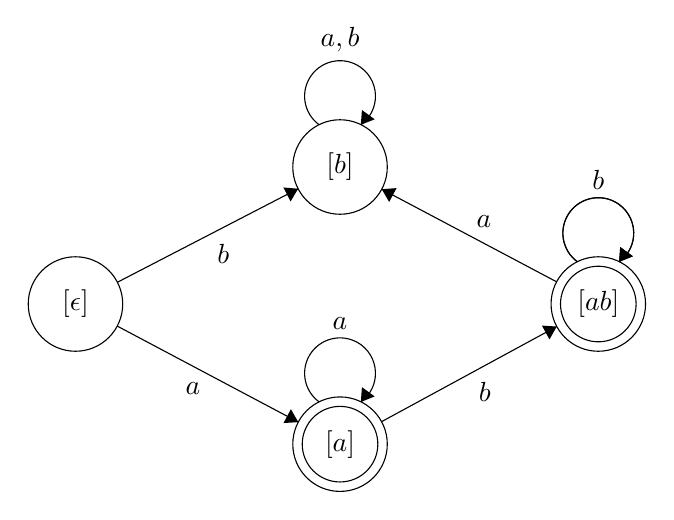
\begin{tikzpicture}[scale=0.2]
\tikzstyle{every node}+=[inner sep=0pt]
\draw [black] (24.4,-28.8) circle (3);
\draw (24.4,-28.8) node {$[\epsilon]$};
\draw [black] (41.2,-20.1) circle (3);
\draw (41.2,-20.1) node {$[b]$};
\draw [black] (41.2,-37.7) circle (3);
\draw (41.2,-37.7) node {$[a]$};
\draw [black] (41.2,-37.7) circle (2.4);
\draw [black] (57.6,-28.8) circle (3);
\draw (57.6,-28.8) node {$[ab]$};
\draw [black] (57.6,-28.8) circle (2.4);
\draw [black] (27.05,-30.2) -- (38.55,-36.3);
\fill [black] (38.55,-36.3) -- (38.08,-35.48) -- (37.61,-36.36);
\draw (31.86,-33.75) node [below] {$a$};
\draw [black] (27.06,-27.42) -- (38.54,-21.48);
\fill [black] (38.54,-21.48) -- (37.6,-21.4) -- (38.06,-22.29);
\draw (33.79,-24.95) node [below] {$b$};
\draw [black] (39.877,-17.42) arc (234:-54:2.25);
\draw (41.2,-12.85) node [above] {$a,b$};
\fill [black] (42.52,-17.42) -- (43.4,-17.07) -- (42.59,-16.48);
\draw [black] (43.84,-36.27) -- (54.96,-30.23);
\fill [black] (54.96,-30.23) -- (54.02,-30.17) -- (54.5,-31.05);
\draw (50.4,-33.75) node [below] {$b$};
\draw [black] (39.877,-35.02) arc (234:-54:2.25);
\draw (41.2,-30.45) node [above] {$a$};
\fill [black] (42.52,-35.02) -- (43.4,-34.67) -- (42.59,-34.08);
\draw [black] (56.277,-26.12) arc (234:-54:2.25);
\draw (57.6,-21.55) node [above] {$b$};
\fill [black] (58.92,-26.12) -- (59.8,-25.77) -- (58.99,-25.18);
\draw [black] (56.277,-26.12) arc (234:-54:2.25);
\fill [black] (58.92,-26.12) -- (59.8,-25.77) -- (58.99,-25.18);
\draw [black] (54.95,-27.39) -- (43.85,-21.51);
\fill [black] (43.85,-21.51) -- (44.32,-22.32) -- (44.79,-21.44);
\draw (50.34,-23.95) node [above] {$a$};
\end{tikzpicture}
\end{center}


Rzeczywiście, jest to automat deterministyczny rozpoznający powyższy język. Zatem minimalny automat ma 4 stany.
\end{example}

\subsection{Lemat o pompowaniu dla języków regularnych}

Przypuśćmy, że język $L \subseteq A^*$ jest regularny. Wówczas istnieje taka stała 
$N \in \mathbb{N}$, że dla każdego słowa $w \in L$ długości co najmniej $N$ istnieje
dekompozycja $w = w_1 \cdot w_2 \cdot w_3$ o następujących własnościach:
\begin{itemize}
    \item słowo $w_2$ jest niepuste,
    \item $|w_1 \cdot w_2| \leq N$,
    \item dla dowolnej liczby naturalnej $k \geq 0$ słowo $w_1 \cdot w_2^k \cdot w_3$
    należy do języka $L$.
\end{itemize}

\begin{example} 
    Pokażemy, że język $L = \{ a^nb^n \mid n \geq 0 \}$ nie jest regularny.
    Przypuśćmy przeciwnie. Wówczas istnieje stała $N \in \mathbb{N}$, 
    o której mowa w lemacie o pompowaniu. Rozważmy słowo $w = a^N b^N$. 
    To słowo należy do języka $L$, więc istnieje dekompozycja $w = w_1 \cdot w_2 \cdot w_3$,
    taka, że $w_2 \neq \epsilon$, $w_1 \cdot w_2^k \cdot w_3 \in L$ dla $k \geq 0$,
    oraz $|w_1 \cdot w_2| \leq N$. Wynika stąd, że słowo $w_2$ zawiera wyłącznie litery $a$
    oraz jest niepuste. Słowo $w_1 \cdot w_2 \cdot w_3$ zawiera więcej liter $a$ niż liter $b$,
    więc nie należy do języka $L$, co jest sprzecznością. Otrzymana sprzeczność pokazuje, że język
    $L$ nie jest regularny.
\end{example}

\begin{problems}
\prob Rozważmy wyrażenie regularne $K=A^* bb A^* + A^* a A A + A^* a A$ nad alfabetem $\{a,b\}$ (zapis $A$ w wyrażeniu to skrót na $(a + b)$). Niech $L$ to język tego wyrażenia. Wtedy
    \answers{automat minimalny dla $L$ ma co najwyżej $4$ stany}{automat minimalny dla $L$ ma przynajmniej $6$ stanów}{istnieje automat niedeterministyczny dla $L$ o $5$ stanach}
    
\prob Dany jest język regularny $L$ dany wyrażeniem regularnym $(a+b)^*a(a+b)(a+b)$. Wówczas
    \answers{każdy automat deterministyczny rozpoznający $L$ ma co najmniej 9 stanów}{minimalny automat deterministyczny rozpoznający $L$ ma 7 stanów}{każdy automat niedeterministyczny rozpoznający $L$ ma co najmniej 6 stanów}
    
\prob Regularny jest język nad alfabetem $\{a,b\}$ złożony ze wszystkich słów, w których każde podsłowo
    \answers{długości 3 występuje parzystą liczbę razy}{długości większej niż 3 występuje parzystą liczbę razy}{występuje również jako prefiks}
\prob Regularny jest język złożony ze wszystkich słów nad alfabetem $\{a,b,c\}$, które
    \answers{zaczynają się od $baca$}{nie zawierają $baca$ jako podsłowa}{zawierają $baca$ jako podsłowo parzystą liczbę razy}   
    
\prob $L$ jest regularny. Czy regularny jest:
    \answers{$\{w: w \in L \land w \in L^R\}$}{$\{ww: w \in L\}$}{prefiksy słów z $L$ parzystej długości}

\prob Językiem regularnym jest
    \answers{język $L \subseteq \{1\}^*$ składający się z unarnych reprezentacji liczb pierwszych}{język $L \subseteq \{0, 1\}^*$ składający się ze słów, w których liczba wystąpień cyfry $0$ przystaje modulo $2$ do liczby wystąpień cyfry $1$}{język $L \subseteq \{0, 1\}^*$ składający się z binarnych reprezentacji liczb podzielnych przez $7$}
\end{problems}

% Michał
\section{Języki bezkontekstowe}
\textbf{Gramatyka bezkontekstowa} $\mathcal{G}$ ma następujące składniki:
\begin{itemize}
    \item Zbiór \textit{terminali} $A$,
    \item Zbiór \textit{nieterminali} $N$, rozłączny z $A$,
    \item Zbiór \textit{produkcji} postaci $q \to w$, gdzie $q \in N$ oraz $w \in (A \cup N)^*$
    jest słowem składającym się z terminali i/lub nieterminali.
    \item Symbolu \textit{startowego} $S$
\end{itemize}

\textbf{Drzewem parsowania} takiej gramatyki jest drzewo etykietowane, w którym:
\begin{itemize}
    \item etykieta korzenia to symbol startowy $S$
    \item liście etykietowane są terminalami ze zbioru $A \cup \{ \epsilon \}$,
    \item wierzchołki wewnętrzne etykietowane są nieterminalami ze zbioru $N$,
    \item jeżeli wierzchołek wewnętrzny ma etykietę $q$, to ma $k$ dzieci o etykietach $s_1, \dots, s_k \in (N \cup A)$ (czytając od lewej do prawej) oraz $q \to s_1 s_2 \dots s_k$ jest produkcją gramatyki (wyjątek: zamiast $k = 0$ robimy dziecko o etykiecie $\epsilon$)
\end{itemize}

\textit{Plon drzewa} to słowo utworzone z etykiet liści, czytanych od lewej do prawej.

\begin{example}
    Rozważmy gramatykę $\mathcal{G}$  o terminalach $a$ oraz $b$, nieterminalu $S$ oraz produkcjach
    $$S \to aSa \; | \; bSb \; | \; a \; | \; b \; | \; \epsilon$$

    Drzewo parsowania dla słowa $abbba$:
    \begin{center}
    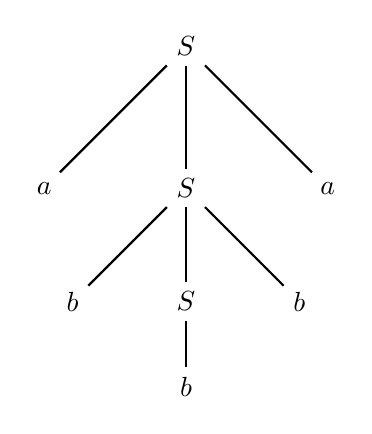
\begin{tikzpicture}[x=1.8cm,y=1.8cm]
        \node (1) at (1.0, 5.0) {$S$}; 
        \node (2) at (0.0, 4.0) {$a$}; 
        \node (3) at (1.0, 4.0) {$S$}; 
        \node (4) at (2.0, 4.0) {$a$}; 
        \node (5) at (0.2, 3.2) {$b$};
        \node (6) at (1.0, 3.2) {$S$};
        \node (7) at (1.8, 3.2) {$b$};
        \node (8) at (1.0, 2.6) {$b$};
        
        \path[-,draw,thick]
            (1) edge (2)
            (1) edge (3)
            (1) edge (4)
            (3) edge (5)
            (3) edge (6)
            (3) edge (7)
            (6) edge (8)
        ;
    \end{tikzpicture}
    \end{center}
    
    Przez indukcję po rozmiarze drzewa parsowania widać, że plonem każdego drzewa parsowania jest palindrom, tj. takie słowo $w$, że $w = w^R$. Odwrotna inkluzja również zachodzi, co możemy udowodnić (ponownie przez indukcję) konstruując drzewo parsowania dla każdego palindromu. Tak więc, $L(\mathcal{G})$ to język palindromów nad alfabetem $\{a, b\}$.
\end{example}

\begin{lemma}
    Każdy język regularny jest bezkontekstowy.
\end{lemma}
Szkic dowodu: dla każdego automatu, da się skonstruować gramatykę, która mu odpowiada.

\subsection{Lemat o pompowaniu dla języków bezkontekstowych}
\begin{lemma} 
    Przypuśćmy, że język $L \subseteq A^*$ jest bezkontekstowy.
    Wtedy istnieje takie $N \in \mathbb{N}$, że każde
    słowo $w \in L$ długości co najmniej $N$ posiada 
    faktoryzację
    $$w = prefix \cdot left \cdot infix \cdot right \cdot suffix$$
    o następujących własnościach:
    \begin{itemize}
        \item słowo $left \cdot right$ jest niepuste
        \item słowo $left \cdot infix \cdot right$
        ma długość co najwyżej $N$
        \item dla każdego $k \geq 0$ słowo
        $w_k = prefix \cdot left^k \cdot infix \cdot right^k \cdot suffix$ należy do języka $L$.
    \end{itemize}
\end{lemma}

\begin{example}
    Pokażemy, że język $L = \{ a^n b^n c^n \mid n \geq 0 \} \subseteq \{a, b, c\}^n$
    nie jest bezkontekstowy. Przypuśćmy przeciwnie. Wtedy istnieje stała $N \in \mathbb{N}$ o której mowa w lemacie o pompowaniu. 
    Rozważmy słowo $w = a^N b^N c^N$ i jego faktoryzację.
    Gdyby $left$ zawierał dwie różne litery 
    (tj. $a$ i $b$, lub $a$ i $c$, lub $b$ i $c$), to słowo $w_2$ nie mogłoby
    należeć do języka $L$. Zatem, $left$ używa tylko jednej litery i analogicznie $right$. 
    Zatem jedna z liter $a$, $b$, $c$, nazwijmy ją $x$, 
    nie pojawia się ani w słowie $left$, ani w słowie $right$. 
    Ponieważ przynajmniej jedno ze słów $left$, $right$ jest niepuste, 
    to jakaś litera $y$ różna od $x$ pojawia się w $left$ lub $right$. 
    Słowo $w_2$ ma więc więcej wystąpień litery $y$ niż litery $x$, 
    więc $w_2 \notin L$. To przeczy tezie lematu o pompowaniu. Tak
    więc, język L nie jest bezkontekstowy.

    Zauważmy, że język $L$ jest przecięciem dwóch języków bezkontekstowych:
    $\{ a^n b^n c^m : n, m \geq 0 \}$ oraz 
    $\{ a^n b^m c^m : n, m \geq 0 \}$
    To przykład na to, że języki bezkontekstowe nie są zamknięte na przecięcia,
    a w konsekwencji nie są też zamknięte na dopełnienie.
\end{example}

Języki bezkontekstowe są zamknięte na:
\begin{itemize}
    \item sumę, konkatenację, gwiazdkę Kleene'go, odwrócenie,
    \item przecięcia z językami regularnymi -- jeśli $L$ jest językiem bezkontekstowym, a $K$ jest językiem regularnym,
    to $L \cap K$ jest językiem bezkontekstowym.
\end{itemize}

% Filip
\subsection{Automaty ze stosem}
Języki bezkontekstowe są rozpoznawane przez pewien rodzaj automatów, nazywanych \textit{automatami ze stosem}. Są one uogólnieniem NFA z $\epsilon$-przejściami, ale z dodatkowym \textit{stosem}. Automat taki ma następujące składniki:
\begin{itemize}
    \item Alfabet wejściowy $A$,
    \item Alfabet stosowy $\Gamma$ zawierający symbol \ dna stosu,
    \item Zbiór stanów $Q$,
    \item Zbiór stanów początkowych $I \subseteq Q$,
    \item Zbiór stanów akceptujących $F \subseteq Q$,
    \item Zbiór przejść $\delta$, gdzie każde jest postaci:
    \[
    p \xrightarrow{ \textbf{pop}(Z),a,\textbf{push}(\gamma) } q
    \]
    dla pewnych $p,q \in Q$, $a \in A \cup \{\epsilon\}$, $Z \in \Gamma$, $\gamma \in \Gamma^*$.
\end{itemize}

Oczywiście \textbf{pop($Z$)} usuwa literę $Z$ z góry stosu, zaś \textbf{push($\gamma$)} wrzuca na stos słowo $\gamma$ (zakładamy, że wrzucenie całego słowa na stos działa tak samo jak wrzucanie po kolei liter od pierwszej do ostatniej -- innymi słowy, stos rośnie w prawo i \textbf{push} dokleja słowo do stosu).

Ważne fakty o automatach ze stosem:
\begin{itemize}
    \item Automaty ze stosem mają tę samą siłę wyrazu co języki bezkonstekstowe,
    \item Zamiast rozważać stany akceptujące można rozważać model, w którym akceptacja zachodzi wtedy, gdy stos jest pusty -- te dwa modele są równoważne,
    \item Każdy automat ze stosem można przerobić na równoważny, mający tylko jeden stan i akceptujący poprzez pusty stos.
\end{itemize}

\begin{problems}

\prob Załóżmy, że $L$ to język bezkontekstowy, zaś $K$ to język regularny, oba nad alfabetem $A$. Przez $X^R$ oznaczamy język powstały z $X$ przez odwrócenie wszystkich słow z $X$. Językiem bezkontekstowym jest język
    \answers{$L^R \cap K$}{$(A^{*} - L) \cup K^*$}{$L^{*} \cup K^R$}

\prob Dane są język bezkontekstowy $L$ i język regularny $K$. Prawdą jest, że
    \answers{$K \backslash L$ jest bezkontekstowy}{$K \cap L$ jest regularny}{$L \backslash K$ jest bezkontekstowy}

\prob Niech $L$ będzie nieskończonym językiem bezkontekstowym nad skończonym alfabetem. Wówczas
    \answers{$L$ jest regularny}{$L$ zawiera nieskończony język regularny}{$L$ zawiera słowo postaci $uv^{2020}xy^{2020}z$, gdzie $vy \neq \epsilon$}

\prob Niech $L$, $K$ to języki bezkontekstowe. Bezkontekstowy wtedy też jest język
    \answers{$L \cup K$}{$L \cap K$}{$L \cap a^*b^*$}

\prob Dla języka $L$, niech $\Psi(L)$ oznacza zbiór długości słów z języka $L$. Istnieje taki język bezkontekstowy $L$, dla którego $\Psi(L)$ jest zbiorem
    \answers{liczb naturalnych podzielnych przez 11}{kwadratów liczb naturalnych}{sześcianów liczb naturalnych}

\prob $L_1$ i $L_2$ są językami bezkontekstowymi nad alfabetem $\Sigma$. Wynika z tego, że bezkontekstowy jest język
    \answers{$L_1\cap L_2$}{$\Sigma^*-L_1$}{$L_1\cup L_2$}    
\prob $L$ jest językiem bezkontekstowym. Wynika z tego, że bezkontekstowy jest język
    \answers{$\{v$ : istnieje słowo z $L$, które można otrzymać przez usunięcie parzystej liczby (niekoniecznie kolejnych) liter z $v\}$}{$\{ww : w \in L\}$}{$\{a_1 \cdots a_n : a_n \cdots a_1 \in L\}$ (tzn. słowa z $L$ pisane do tyłu)}
    
\prob Następujący język jest bezkontekstowy:
    \answers
    {$\{a^nb^mc^kd^l : n = k \text{ i } m = l\}$}
    {$\{a^nb^mc^kd^l : n = l \text{ i } m = k\}$}
    {$\{a^nb^mc^kd^l :n=m \text{ i } k=l\}$}
    
\prob Jeśli $L_1$ jest językiem bezkontekstowym, a $L_2$ jest językiem regularnym, to bezkontekstowy jest język
    \answers
    {$L_1 \cap L_2$}
    {$\{vw : v \in L_1, w \in L_2\}$}
    {$\{v^R : v \in L_1\}$, gdzie $v^R$ oznacza odwrócenie słowa $v$}

\prob Zbiór dziesiętnych zapisów liczb podzielnych przez 7 jest
    \answers
    {językiem regularnym}
    {językiem bezkontekstowym}
    {językiem kontekstowym}
\end{problems}

% Jasiek
\section{Języki obliczalne}
\textbf{Maszyna Turinga} to krotka $M = \langle A, B, Q, q_I, q_F, \delta \rangle$, gdzie:
\begin{itemize}
    \item $A$ - alfabet wejściowy
    \item $B$ - alfabet roboczy (taki, którym posługuje się maszyna)
    \item $Q$ - skończony zbiór stanów
    \item $q_I$ - stan początkowy
    \item $q_F$ - stan końcowy
    \item $\delta$ - funkcja przejścia, gdzie $\delta: Q \times B \to B \times \{\xleftarrow{}, \xrightarrow{} \} \times Q$
\end{itemize}
Charakterystyka podstawowej maszyny Turinga:
\begin{itemize}
    \item działa na jednostronnie nieskończonym ciągu komórek nazywanym \textbf{taśmą}
    \item posiada głowicę poruszającą się wzdłuż taśmy
    \item głowica wskazuje na aktualnie rozważaną komórkę taśmy
    \item może wykonać tranzycję $t = (p, a, b, d, q)$ w następujący sposób:
    \begin{itemize}
        \item maszyna znajduje się w stanie $p$
        \item w aktualnie rozważanej komórce znajduje się litera $a$
        \item wykonując tranzycję w miejsce litery $a$ wpisana zostaje litera $b$
        \item głowica zostaje przesunięta w kierunku $d \in \{\xleftarrow{}, \xrightarrow{}\}$
        \item maszyna przechodzi do stanu $q$
    \end{itemize}
\end{itemize}
Intuicyjnie maszyna Turinga $M$ jest w stanie sprawdzać swój aktualny stan i na jego podstawie decydować, co zamierza zrobić dalej, być może zmieniając zawartość taśmy. Po więcej szczegółowych definicji odsyłam do \href{https://www.mimuw.edu.pl/~szymtor/jao/skrypt.pdf#chapter.4}{skryptu}.

\textbf{Równoważne warianty maszyn Turinga:}
\begin{itemize}
    \item zwykła maszyna Turinga opisana powyżej;
    \item maszyna Turinga z binarnym alfabetem roboczym ($B = \{0, 1, \_\}$);
    \item maszyna Turinga z taśmą nieskończoną w obu kierunkach;
    \item maszyna Turinga z wieloma taśmami;
    \item niedeterministyczna maszyna Turinga.
\end{itemize}

\textbf{Funkcje obliczalne:} oznaczmy przez $L(M)$ zbiór słów $w \in A^*$, na których maszyna $M$ terminuje. Oznaczmy przez $f_M(w): A^* \to B^*$ funkcję częściową, która słowu $w \in L(M)$ przyporządkowuje wynik obliczenia $M$ na $w$, a dla pozostałych słów jest nieokreślona. Mówimy, że $M$ oblicza funkcję $f_M$. Funkcja częściowa $f: A^* \to B^*$ jest \textbf{obliczalna} jeśli istnieje maszyna Turinga, która ją oblicza.

\begin{example}
    Rozważmy słowa $w \in \{0, 1\}^*$ reprezentujące grafy. Funkcja $f$ ma za zadanie zwrócić jeden wtedy i tylko wtedy, gdy $w$ jest opisem grafu spójnego. Taka funkcja $f$ jest obliczalna, ponieważ możemy zasymulować na taśmie maszyny Turinga algorytm BFS (zapisując m. in. zbiór odwiedzonych wierzchołków i wykonując odpowiednie przejścia).
\end{example}

Język $L \subseteq A^*$ jest \textbf{obliczalny}, jeżeli jego funkcja charakterystyczna jest obliczalna. Jeżeli język $L$ jest obliczalny, to odpowiadający mu problem decyzyjny jest \textbf{rozstrzygalny}. Innymi słowami problem decyzyjny jest rozstrzygalny jeśli istnieje algorytm, który dla każdego słowa wejściowego $w$ terminuje oraz odpowiada "TAK" lub "NIE" w zależności od tego czy $w \in L$. Przykładem języków obliczalnych są języki regularne oraz bezkontekstowe. Języki obliczalne są zamknięte na:
\begin{itemize}
    \item sumy;
    \item przecięcia;
    \item dopełnienia.
\end{itemize}

Język $L \subseteq A^*$ jest \textbf{częściowo obliczalny}, jeżeli istnieje maszyna Turinga, która terminuje dla wszystkich słów $w \in L$, a dla słów $w' \in A^* - L$ nie terminuje. Jeżeli język $L$ jest częściowo obliczalny, to odpowiadający mu problem decyzyjny jest \textbf{półrozstrzygalny}. Innymi słowami problem decyzyjny jest półrozstrzygalny jeśli istnieje algorytm, który dla każdego słowa wejściowego $w$ odpowiada "TAK" wtedy i tylko wtedy, gdy $w \in L$, a w przeciwnym wypadku się wiesza. Każdy język obliczalny jest też częściowo obliczalny. Języki częściowo obliczalne są zamknięte na:
\begin{itemize}
    \item sumy;
    \item przecięcia.
\end{itemize}

\textbf{Lemat 1.} {\it Język $L \subseteq A^*$ jest obliczalny wtw. gdy $L$ oraz $A^* - L$ są częściowo obliczalne.}

\textbf{Lemat 2.} {\it Języki częściowo obliczalne to dokładnie klasa języków rozpoznawanych przez maszyny Turinga.}

\textbf{Problem stopu} -- inaczej nazywany problemem \textbf{HALT} -- dla danej maszyny Turinga $M$ oraz słowa $w$ stwierdź, czy $M$ terminuje na $w$. Do języka HALT należą więc wszystkie pary $\langle M, w \rangle$ takie, że $M$ terminuje na $w$. Język HALT jest częściowo obliczalny (ale nie jest obliczalny). Dopełnienie języka HALT nie jest częściowo obliczalne.

Przydatnym wariantem powyższego problemu jest problem HALT$_\epsilon$, czyli język maszyn Turinga terminujących na słowie pustym. Nie jest on obliczalny. Aby to udowodnić, wykorzystamy metodę \textbf{redukcji}.

\begin{example}
    Załóżmy, że dana jest maszyna $M$ oraz słowo wejściowe $w$. Niech nowa maszyna $M_w$ działa w następujący sposób: $M_w$ wymazuje swoje wejście zastępując je słowem $w$, a następnie symuluje działanie $M$ na $w$. Maszyna $M_w$ zatrzyma się na słowie pustym wtw. gdy $M$ zatrzyma się na słowie $w$. Zatem
    \begin{itemize}
        \item dla danego kodu $k$ maszyny $M$ oraz słowa $w \in A^*$ istnieje kod $k_w$, że $k \in \text{ HALT} \Leftrightarrow k_w \in \text{ HALT}_\epsilon$
        \item funkcja $(k, w) \to k_w$ jest obliczalna
    \end{itemize}
    Z tego wynika, że HALT$_\epsilon$ nie jest obliczalny.
\end{example}

Formalnie, \textbf{redukcja} problemu $L \subseteq A^*$ do problemu $K \subseteq B^*$ to funkcja $f: A^* \to B^*$ taka, że $\forall w \in A^*$ zachodzi $w \in L \Leftrightarrow f(w) \in K$. Redukcja $f$ jest obliczalna jeżeli $f$ jest obliczalna. Oznacza to w szczególności, że jeżeli istnieje redukcja obliczalna języka $L$ do $K$ oraz $K$ jest obliczalny, to $L$ również jest obliczalny.

Znane problemy nierozstrzygalne:
\begin{itemize}
    \item problem stopu
    \item czy język bezkontekstowy $L$ rozpoznaje każde słowo $w \in A^*$?
    \item czy język bezkontekstowy $L$ zawiera się w języku bezkontekstowym $K$?
\end{itemize}

% Jasiek
\section{Klasy P, NP oraz NP-zupełność}
Język $L$ jest w klasie P jeżeli istnieje \textbf{deterministyczna} maszyna Turinga $M$ oraz wielomian $f: \NN \to \NN$ takie, że:
\begin{itemize}
    \item L(M) = L;
    \item dla każdego słowa $w \in A^*$ maszyna $M$ wykonuje co najwyżej $f(|w|)$ kroków na słowie $w$.
\end{itemize}
Mniej formalnie: $L \in$ P jeżeli istnieje algorytm rozwiązujący problem $L$ w czasie wielomianowym.

Język $L$ jest w klasie NP jeżeli istnieje \textbf{niedeterministyczna} maszyna Turinga $M$ oraz wielomian $f: \NN \to \NN$ takie, że:
\begin{itemize}
    \item L(M) = L;
    \item dla każdego słowa $w \in A^*$, każdy bieg maszyny $M$ po słowie $w$ wykonuje co najwyżej $f(|w|)$ kroków.
\end{itemize}

Oczywiście P $\subseteq$ NP, ale czy NP $\subseteq$ P? Jest to bardzo ważny problem otwarty. Wiemy natomiast, że równoważne są warunki:
\begin{itemize}
    \item P = NP
    \item któryś z problemów z poniższej listy należy do klasy P
    \item każdy z problemów z poniższej listy należy do do klasy P
\end{itemize}

Lista niektórych problemów NP-zupełnych:
\begin{itemize}
    \item CNF-SAT \\
    To problem spełnialności formuł w postaci CNF, a więc koniunkcji wielu klauzul, gdzie klauzula jest alternatywą literałów. Literał to zmienna lub negacja zmiennej.
    \item 3CNF-SAT \\
    Instancja problemu CNF-SAT, w której każda klauzula składa się z maksymalnie trzech literałów.
    \item Ścieżka Hamiltona (analogicznie cykl Hamiltona) \\
    Czy w zadanym grafie istnieje ścieżka, która odwiedza każdy z wierzchołków grafu dokładnie raz?
    \item Problem kliki \\
    Czy dany graf zawiera klikę rozmiaru $k$?
    \item Zbiór niezależny \\
    Czy istnieje zbiór mocy $k$ złożony z wierzchołków zadanego grafu $G$ taki, że żadne dwa wierzchołki nie są połączone krawędzią w $G$?
    \item 3-kolorowanie grafu \\
    Czy da się pokolorować wierzchołki grafu na 3 kolory w taki sposób, że żadna krawędź nie łączy dwóch wierzchołków o tym samym kolorze?
    \item akceptacja pustego słowa \\
    Dana niedeterministyczna maszyna Turinga $M$ oraz liczba $n$, czy $M$ akceptuje słowo puste w co najwyżej $n$ krokach?
\end{itemize}

Aby dowieść, że problem $P$ jest NP-zupełny przeprowadzamy \textbf{redukcję wielomianową} z innego, znanego problemu NP-trudnego:
\begin{enumerate}
    \item Uzasadnij, że $P$ jest w klasie NP.
    \item Zredukuj przy pomocy redukcji wielomianowej znany problem NP-trudny do problemu $P$.
    \item $P$ jest w klasie NP i jest NP-trudny $\implies$ $P$ jest NP-zupełny.
\end{enumerate}

Zauważmy, że problem może być NP-trudny (to znaczy co najmniej tak trudny jak inne problemy NP-trudne) nie będąc NP-zupełnym. Jest tak na przykład z problemem stopu.

\begin{example}
    Założmy, że wiemy, że problem 3-kolorowania grafu (3-KOL) jest NP-trudny. Pokażemy, że problem 3-CNF-SAT jest NP zupełny.
    \begin{enumerate}
        \item 3-CNF-SAT jest w klasie NP, ponieważ możemy niedeterministycznie zgadnąć wartościowanie zmiennych, a następnie w czasie wielomianowym sprawdzić, czy formuła logiczna jest spełniona.
        \item Niech $G = (V, E)$ będzie wejściem dla problemu 3-KOL. Dla każdego $v \in V$ tworzymy zmienną $x_v^i, \; i \in \{1, 2, 3\}$ oznaczającą, że wierzchołek $v$ ma kolor $i$. Oczywiście każdy wierzchołek musi mieć przyporządkowany dokładnie jeden kolor, więc tworzymy klauzule:
        \begin{align*}
            \forall_{v \in V} (x_v^1 \lor x_v^2 \lor x_v^3) \land (\neg x_v^1 \lor \neg x_v^2) \land (\neg x_v^1 \lor \neg x_v^3) \land (\neg x_v^2 \lor \neg x_v^2)
        \end{align*}
        Dodatkowo dla każdej krawędzi chcemy, by kolory incydentnych do niej wierzchołków nie były równe:
        \begin{align*}
            \forall_{e = (v, u) \in E} \forall_{i \in \{1, 2, 3\}} (\neg x_v^i \lor \neg x_u^i)
        \end{align*}
        W ten sposób otrzymujemy formułę $\phi$ w postaci 3-CNF. Gdybyśmy potrafili rozwiązać problem 3-CNF-SAT dla $\phi$, to potrafilibyśmy rozwiązać problem 3-KOL dla $G = (V, E)$ przepisując wartościowanie zmiennych na odpowiednie kolory. Taka redukcja jest \textbf{wielomianowa} - dla każdego wierzchołka i krawędzi oryginalnego grafu wykonujemy wielomianową (stałą) liczbę operacji.
        \item 3-CNF-SAT jest w klasie NP oraz jest NP-trudny, a zatem jest NP-zupełny.
    \end{enumerate}
\end{example}

\begin{problems}
\prob Język $L = \{a^nb^n \mid n \in \mathbb{N}\}$ jest
    \answers{regularny}{bezkontekstowy}{obliczalny w czasie wielomianowym}

\prob Zbiór dziesiętnych zapisów potęg dwójki jest
    \answers{językiem bezkontekstowym}{językiem należącym do klasy P}{językiem należącym do klasy NP}

\prob Zakładamy, że język regularny jest dany jako automat niedeterministyczny, a język bezkontekstowy jako gramatyka bezkontekstowa. Problemem rozstrzygalnym jest stwierdzenie
    \answers{czy dany język bezkontekstowy jest zawarty w danym języku bezkontekstowym}{czy dany język bezkontekstowy jest zawarty w danym języku regularnym}{czy dany język regularny jest zawarty w danym języku bezkontekstowym}

\prob Dla dowolnego języka $L \subseteq A^*$ nad alfabetem $A$ oznaczmy przez $L^R$ zbiór ,,lustrzanych odbić'' słów z $L$. Formalnie: $$\epsilon^R = \epsilon, \quad (wa)^R = a(w^R) \text{ dla } a \in A, w \in A^*, \quad L^R = \{w^R : w \in L\}.$$ Niech $L' = LL^R$ oznacza konkatenację języków $L$ i $L^R$. Wynika z tego, że
    \answers
    {jeżeli $L$ jest regularny, to $L'$ też}
    {jeżeli $L$ jest bezkontekstowy, to $L'$ też}
    {jeżeli $L$ jest rozstrzygalny, to $L'$ też}

\prob Problemem rozstrzygalnym jest stwierdzenie
    \answers
    {czy gramatyka bezkontekstowa generuje język regularny}
    {czy możemy rozpoznać słowo puste na maszynie Turinga $\mathcal{M}$ w mniej niż $n$ kroków}
    {czy deterministyczna maszyna Turinga w $f(n)$ krokach rozpozna wszystkie słowa długości $n$ dla każdego $n$}
    
 \prob Dany jest alfabet $A = \{a, b\}$ oraz
    \begin{itemize}
        \item język bezkontekstowy $K$ nad $A$ dany jako gramatyka,
        \item język regularny $R$ nad $A$ dany jako niedeterministyczny automat.
    \end{itemize}
    Problemem rozstrzygalnym jest
    \answers{określenie niepustości podzbioru $R$ takich słów, dla których liczba liter $a$ jest równa liczbie liter $b$}{sprawdzenie, że $K \subset R$}{sprawdzenie, że $R \subset K$}
    
    \prob Problem stopu dla maszyn Turinga jest
    \answers{w klasie NP}{częściowo rozstrzygalny}{rozstrzygalny}
\end{problems}

\begin{solutions}

    % Filip
    \sol Rozważmy wyrażenie regularne $K=A^* bb A^* + A^* a A A + A^* a A$ nad alfabetem $\{a,b\}$ (zapis $A$ w wyrażeniu to skrót na $(a + b)$). Niech $L$ to język tego wyrażenia. Wtedy
    \answerss{automat minimalny dla $L$ ma co najwyżej $4$ stany}{automat minimalny dla $L$ ma przynajmniej $6$ stanów}{istnieje automat niedeterministyczny dla $L$ o $5$ stanach}{TAK}{NIE}{TAK}

    Znajdziemy klasy abstrakcji przy relacji Myhilla-Nerodego. 
    
    \textit{Uwaga.} Dalej w rozwiązaniu będziemy skrótowo mówić o słowie $w$, na przykład, że słowo $w$ ,,rozróżnia'' dane klasy abstrakcji -- chodzić będzie zawsze o $w$ z definicji relacji Myhilla-Nerodego.
    
    Pierwszą oczywiście będzie $[\epsilon]$. Jako następną sprawdzimy $[a]$. Są to różne klasy abstrakcji, bo dla $w = a$ mamy różne przyszłości -- $\epsilon w$ nie akceptuje, zaś $a w$ tak. Sprawdźmy $[b]$. Jest to klasa różna od $[\epsilon]$ -- rozróżnia je na przykład $w = b$. Klasy $[b]$ i $[a]$ rozróżnia $w = a$. Zatem jest to nowa klasa różna od poprzednich. Następnie sprawdźmy klasę $[aa]$. Klasę tę rozróżnia od każdej poprzedniej przyszłość $w = \epsilon$. 
    
    Zanim kontynuujemy poszukiwania zauważmy istotną obserwację: język $L$ zawiera wszystkie słowa długości co najmniej 3 (warto sprawdzić samemu dlaczego -- wystarczy przyjrzeć się trzem ostatnim literom przykładowego słowa) i prawie wszystkie długości 2 -- nie zawiera tylko słowa $ba$. Stąd wynika, że wszystkie klasy abstrakcji postaci $[u]$, gdzie $|u| \geqslant 3$, są sobie równe. Ponadto klasa $[aaa]$ jest równa klasie $[aa]$ (ponieważ $w = \epsilon$ daje ten sam rezultat, a $w \not= \epsilon$ w obu przypadkach prowadzi do słowa długości $\geqslant 3$). To oznacza, że jedyne klasy jakie pozostało sprawdzić, to klasy o dwuliterowych reprezentatach.
    
    Łatwo zauważyć (podobnie do argumentu, że $[aa] = [aaa]$), że $[ab]$ i $[bb]$ również są tą samą klasą co $[aa]$. Z kolei $[ba]$ jest tą samą klasą co $[a]$. Zatem mamy wszystkie klasy: $[\epsilon]$, $[a]$, $[b]$ i $[aa]$. Stąd minimalny automat (deterministyczny) ma 4 stany. W punkcie $\mathbf{C}$ warto pamiętać, że automaty deterministyczne są również w szczególności automatami niedeterministycznymi, a znaleźliśmy 4-stanowy.

    % Michał
    \sol Dany jest język regularny $L$ dany wyrażeniem regularnym $(a+b)^*a(a+b)(a+b)$. Wówczas
    \answerss{każdy automat deterministyczny rozpoznający $L$ ma co najmniej 9 stanów}{minimalny automat deterministyczny rozpoznający $L$ ma 7 stanów}{każdy automat niedeterministyczny rozpoznający $L$ ma co najmniej 6 stanów}{NIE}{NIE}{NIE}    

    Zauważmy, że to wyrażenie regularne, rozpoznaje dokładnie wszystkie słowa, których trzecia literka od końca to $a$.

    Zatem, każdą klasę abstrakcji w relacji Myhilla-Nerodego można utożsamić z ze stanem: na jakich z ostatnich 3 ostatnich
    pozycji znajdują się literki $a$? Nietrudno zauważyć, że jeśli dla dwóch słów, odpowiedź na to pytanie jest różna,
    można znaleźć taki człon, że po doklejeniu go do słów, tylko jedno z nich jest akceptujące.

    Mamy więc $2^3 = 8$ klas abstrakcji, czyli co najmniej 8 stanów w DFA, zatem odpowiedzi w \textbf{A.} oraz \textbf{B.} to NIE.

    \textbf{C.} można skonstruować 5-stanowe NFA. Wyrażenie regularne ma 4 człony ($(a + b)^*$, $a$, $(a + b)$, $(a + b)$),
    $i$-ty ($i \in \{ 0, 1, 2, 3, 4 \}$) stan oznacza, że już rozpoznaliśmy $i$ członów wyrażenia.
    

    % Jasiek
    \sol Regularny jest język nad alfabetem $\{a,b\}$ złożony ze wszystkich słów, w których każde podsłowo
    \answerss{długości 3 występuje parzystą liczbę razy}{długości większej niż 3 występuje parzystą liczbę razy}{występuje również jako prefiks}{TAK}{TAK}{TAK} 
    W \textbf{A.} tworzymy automat, który dla każdego z ośmiu możliwych słów długości 3 pamięta dla każdego z nich parzystość jego występowań jako podsłowo. Akceptacja ma miejsce w stanie odpowiadającym samym parzystym wystąpieniom. W \textbf{B.} korzystamy z następującej obserwacji: jednym z podsłów słowa $w$ jest całe słowo $w$. Oczywiście pojawia się ono jako podsłowo dokładnie raz, a więc nieparzystą liczbę razy. Język ten składa się więc ze słów o mniej niż 3 literach, więc jest regularny. W \textbf{C.} zauważamy, że do języka należą tylko słowa złożone z samych liter $a$ lub samych liter $b$. Jest on oczywiście regularny ($L = a^* + b^*$).

    % Michał
    \sol Regularny jest język złożony ze wszystkich słów nad alfabetem $\{a,b,c\}$, które
    \answerss{zaczynają się od $baca$}{nie zawierają $baca$ jako podsłowa}{zawierają $baca$ jako podsłowo parzystą liczbę razy}{TAK}{TAK}{TAK}    

    \textbf{A.} Ten język jest rozpoznawany przez wyrażenie regularne {\ttfamily baca(a+b+c)$^*$}.
    
    \textbf{B.} Stworzymy DFA, który rozpoznaje ten język. Niech stanem będą 4 ostatnie literki słowa. Przejścia konstruujemy w naturalny sposób.
    Usuwamy przejścia ze stanu $baca$, żeby nie akceptować go jako podsłowa.

    \textbf{C.} Znowu będziemy tworzyć DFA. Niech stan będzie postaci:
        $$\langle \text{4 ostatnie literki słowa}, \text{parzystość liczby wystąpień } baca\rangle$$
        Ponownie, konstruujemy przejścia z definicji, i oznaczamy stany z parzystą liczbą wystąpień jako akceptujące.

    % Jasiek
    \sol $L$ jest regularny. Czy regularny jest:
    \answerss{$\{w: w \in L \land w \in L^R\}$}{$\{ww: w \in L\}$}{prefiksy słów z $L$ parzystej długości}{TAK}{NIE}{TAK}
    \textbf{A.} rozważmy przecięcie $L$ z $L^R$. Języki regularne są zamknięte na przecięcia oraz odwracanie, więc odpowiedź jest twierdząca. \\
    \textbf{B.} rozważmy $L = A^*$. Wtedy język z treści to język zduplikowanych słów nad $A$ - nazwijmy go $L'$. Jeśli $L'$ byłby regularny, to jego przecięcie z językiem regularnym $L'' = a^*b^*a^*b^*$ byłoby równe $L' \cap L'' = \{a^nb^ma^nb^m\}$. Ten język oczywiście nie jest regularny (proste pompowanie), a więc ze względu na zamkniętość języków regularnych na przecięcia $L'$ nie mógł być regularny. \\
    \textbf{C.} rozważmy automat $A$ rozpoznający $L$ i stwórzmy na jego podstawie automat $A'$, który dla każdego stanu $s$ automatu $A$ utworzy dwie wersje $s$: $s_0$ oraz $s_1$. Do $s_0$ będziemy mogli się dostać tylko w parzystej liczbie ruchów, a do $s_1$ tylko w nieparzystej (wymaga to zwykłego skopiowania $A$ i dostawienia analogicznych krawędzi łączących stany parzyste z nieparzystymi). Akceptujemy w parzystych wersjach stanów akceptujących $A$.

    % Kasia K
    \sol Językiem regularnym jest
    \answerss{język $L \subseteq \{1\}^*$ składający się z unarnych reprezentacji liczb pierwszych}{język $L \subseteq \{0, 1\}^*$ składający się ze słów, w których liczba wystąpień cyfry $0$ przystaje modulo $2$ do liczby wystąpień cyfry $1$}{język $L \subseteq \{0, 1\}^*$ składający się z binarnych reprezentacji liczb podzielnych przez $7$}{NIE}{TAK}{TAK}

    \begin{enumerate}[\bf A.]
        \item Ze względu na nieskończoność i nieregularność liczb pierwszych automat generujący ten język musiałby być nieskończony.
        \item Automat generujący ten język składa się z 4 stanów poetykietowanych $(\#_0 \mod 2, \#_1 \mod 2)$. Łatwo zauważyć że przejścia są postaci $(x, y) \xrightarrow{0} (1-x, y)$ i $(x, y) \xrightarrow{1} (x, 1- y)$, stan początkowy to $(0, 0)$, a stany akceptujące to $(x,x)$.
        \item Można zauważyć, że kolejne potęgi 2 przy dzieleniu przez 7 dają kolejno reszty 1,2,4. A zatem automat generujący ten język składa się z 21 stanów poetykietowanych $(x, y) : x \in \{0,1,2,3,4,5,6\}\, y \in \{1,2,4\}$. Łatwo zauważyć że przejścia są postaci $(x, y) \xrightarrow{z} ((x + zy) \mod 7, y^2 \mod 7)$, stan początkowy to $(0, 1)$, a stany akceptujące to $(0,x)$.
    \end{enumerate}

    %Patryk
    \sol Załóżmy, że $L$ to język bezkontekstowy, zaś $K$ to język regularny, oba nad alfabetem $A$. Przez $X^R$ oznaczamy język powstały z $X$ przez odwrócenie wszystkich słow z $X$. Językiem bezkontekstowym jest język
    \answerss{$L^R \cap K$}{$(A^{*} - L) \cup K^*$}{$L^{*} \cup K^R$}{TAK}{NIE}{TAK}
    A) $L^R$ jest bezkontekstowy (odwrócenie automatu albo gramatyki), wiemy że przecięcie języka bezkontekstowego z regularnym daje bezkontekstowy.\\
    B) Języki bezkontekstowe nie są zamknięte na dopełnienie.\\
    C) Języki bezkontekstowe są zamknięte na gwiazdkę Kleene'go, a języki regularne na odwrócenia, więc ich suma jest językiem bezkontekstowym.

    %Patryk
    \sol Dane są język bezkontekstowy $L$ i język regularny $K$. Prawdą jest, że
    \answerss{$K \backslash L$ jest bezkontekstowy}{$K \cap L$ jest regularny}{$L \backslash K$ jest bezkontekstowy}{NIE}{NIE}{TAK}
    A) Załóżmy, że $K$ to język zawierające wszystkie słowa nad alfabetem $\{a,b\}$. Wówczas $K-L$ jest dopełnieniem, a przecież języki bezkontesktowe nie są zamknięte na dopełnienie.\\
    B) Takie przecięcie jest bezkontekstowe ale nie regularne.\\
    C) $L-K = L \cap (A^*-K)$. Dopełnienie języka regularnego jest językiem regularnym więc w przecięciu z językiem bezkontekstowym daje język bezkontekstowy.

    %Tomek
    \sol Niech $L$ będzie nieskończonym językiem bezkontekstowym nad skończonym alfabetem. Wówczas
    \answerss{$L$ jest regularny}{$L$ zawiera nieskończony język regularny}{$L$ zawiera słowo postaci $uv^{2020}xy^{2020}z$, gdzie $vy \neq \epsilon$}{NIE}{NIE}{TAK}
    \textbf{A.} Każdy język regularny jest językiem bezkontekstowym, ale nie na odwrót. Np. $ a^n b^n $ \\ 
    \textbf{B.}  Żaden nieskończony podzbiór języka bezkontekstowego $ a^n b^n $ nie będzie językiem regularnym \\ 
    \textbf{C.} Jeśli L jest bezkontekstowy, to zachodzi dla niego lemat o pompowaniu dla j. bezkontekstowych. Biorąc dowolne słowo postaci $uvxyz \in L$,  wiemy że dla $uv \ne \epsilon $  zachodzi $uv^{k}xy^{k}z \in L$, a w szczególności $uv^{2020}xy^{2020}z \in L$. \\
    
    %Tomek
    \sol Niech $L$, $K$ to języki bezkontekstowe. Bezkontekstowy wtedy też jest język
    \answerss{$L \cup K$}{$L \cap K$}{$L \cap a^*b^*$}{TAK}{NIE}{TAK}
    \textbf{A.} Języki bezkontekstowe są zamknięte na sumę. \\ 
    \textbf{B.} Języki bezkontekstowe nie są zamknięte na przecięcia. \\ 
    \textbf{C.} Języki bezkontekstowe są zamknięte na przecięcia językiem regularnym. \\
    


    \sol Dla języka $L$, niech $\Psi(L)$ oznacza zbiór długości słów z języka $L$. Istnieje taki język bezkontekstowy $L$, dla którego $\Psi(L)$ jest zbiorem
    \answerss{liczb naturalnych podzielnych przez 11}{kwadratów liczb naturalnych}{sześcianów liczb naturalnych}{TAK}{NIE}{NIE}
    \textbf{A.} Tak, wystarczy wziąć język $(a^{11})^*$. To język regularny, a języki regularne są w szczególności bezkontekstowe.

    \textbf{B.} Taki język łamałby lemat o pompowaniu. Przypuśćmy, że jest taki język i istnieje dla niego stała $N$ z lematu o pompowaniu. Wtedy weźmy dowolne słowo $w$ o długości $\geq N$. Zauważmy, że pompując to słowo, jego długość rośnie jak ciąg arytmetyczny. Ale odległości pomiędzy kwadratami liczb naturalnych rosną, im większe są te kwadraty, w związku z tym nie jest możliwe, aby ww. pompowanie generowało słowa, których długości zawsze są kwadratami liczb naturalnych.

    \textbf{C.} Analogicznie do \textbf{B.}


    % Julia
    \sol $L_1$ i $L_2$ są językami bezkontekstowymi nad alfabetem $\Sigma$. Wynika z tego, że bezkontekstowy jest język
    \answerss{$L_1\cap L_2$}{$\Sigma^*-L_1$}{$L_1\cup L_2$}{NIE}{NIE}{TAK}
    \textbf{A.} Języki bezkontekstowe nie są zamknięte na przecięcia. \\
    \textbf{B.} Języki bezkontekstowe nie są zamknięte na dopełnienia. \\
    \textbf{C.} Języki bezkontekstowe są zamknięte na sumę.
    
    \sol $L$ jest językiem bezkontekstowym. Wynika z tego, że bezkontekstowy jest język
    \answerss{$\{v$ : istnieje słowo z $L$, które można otrzymać przez usunięcie parzystej liczby (niekoniecznie kolejnych) liter z $v\}$}{$\{ww : w \in L\}$}{$\{a_1 \cdots a_n : a_n \cdots a_1 \in L\}$ (tzn. słowa z $L$ pisane do tyłu)}{TAK}{NIE}{TAK}
    \textbf{A}  \textbf{B} Nie, byłoby tak dla języka $\{ww^R : w \in L \}$, ale tutaj nie możemy się nagle dowiedzieć, że jesteśmy na początku słowa $w$, bo informacja o tym jest na dole stosu. \textbf{C} języki bezkontekstowe są zamknięte na odwrócenia.
    
    \sol Następujący język jest bezkontekstowy:
    \answerss
    {$\{a^nb^mc^kd^l : n = k \text{ i } m = l\}$}
    {$\{a^nb^mc^kd^l : n = l \text{ i } m = k\}$}
    {$\{a^nb^mc^kd^l :n=m \text{ i } k=l\}$}
    {NIE}{TAK}{TAK}    
    \textbf{A.} mamy język $a^nb^kc^nd^k$. Weźmy $N$ z lematu o pompowaniu i słowo $a^{2N}b^{3N}c^{2N}d^{3N}$. Niech $left, \ right$ będą wewnątrz jednej literki. Wtedy psuje się symetria między $a$ i $c$ lub $b$ i $d$. Jeśli $left$ jest w $a$, $right$ zaś w $b$, to także psuje się symetria. Jeśli $left$ lub $right$ są same w sobie na skraju literek, psuje się całkiem układ słowa. Stąd nie jest to język bezkontekstowy. 
    \textbf{B.} język $a^nb^kc^kd^n$ wyraża gramatyka $S \to aRd$, $R\to aRd \ | L$, $L \to bLc \ | \ \varepsilon$.
    \textbf{C.} język $a^nb^nc^kd^k$ wyraża gramatyka $S \to LR$, $L \to aLb \ | \ \varepsilon$, $R \to cRb \ | \varepsilon$.

    % Julia
    \sol Jeśli $L_1$ jest językiem bezkontekstowym, a $L_2$ jest językiem regularnym, to bezkontekstowy jest język
    \answerss
    {$L_1 \cap L_2$}
    {$\{vw : v \in L_1, w \in L_2\}$}
    {$\{v^R : v \in L_1\}$, gdzie $v^R$ oznacza odwrócenie słowa $v$}
    {TAK}{TAK}{TAK}
    \textbf{A.} Języki bezkontekstowe są zamknięte na przecięcia z językami regularnymi. \\
    \textbf{B.} Każdy język regularny jest bezkontekstowy, zatem $L_2$ bezkontekstowy. Języki bezkontekstowe są zamknięte na konkatenację. \\
    \textbf{C.} Języki bezkontekstowe są zamknięte na odwrócenie.

    % Filip
    \sol Zbiór dziesiętnych zapisów liczb podzielnych przez 7 jest
    \answerss
    {językiem regularnym}
    {językiem bezkontekstowym}
    {językiem kontekstowym}
    {TAK}{TAK}{TAK}

    Pokażemy, że jest to język regularny poprzez opis automatu rozpoznającego ten język. Automat ten będzie miał 8 stanów: 7 stanów $q_i$ dla $i \in \{ 0, 1, \ldots, 6 \}$ oznaczających resztę z dzielenia dotychczas wpisanej liczby (stan $q_0$ jest stanem akceptującym), oraz ósmy stan $q_I$, który będzie stanem początkowym -- jest on potrzebny, bo zanim wczytamy pierwszą literę, wczytaliśmy tylko puste słowo, a ono nie reprezentuje żadnej liczby. Przejścia w takim automacie są nastepujące:
    \begin{itemize}
    \item $q_I \xrightarrow{n} q_{n \text{ mod } 7}$ dla $n \in \{ 0, 1, \ldots, 9 \}$,
    \item $q_i \xrightarrow{n} q_j$ wtw. $j \equiv 10i + j \text{ mod } 7$.
    \end{itemize}
    Przejścia z pierwszego punktu to po prostu zapamiętanie reszty z dzielenia przez 7, gdy wczytujemy pierwszą cyfrę. Przejścia z drugiego punktu to update reszty z dzielenia po dopisaniu kolejnej cyfry -- zauważmy, że dopisanie cyfry $k$ do liczby odpowiada pomnożeniu tej liczby przez 10 i dodaniu $k$.

    Języki regularne są również bezkontekstowe i kontekstowe. 
    
    \textit{Uwaga}: języki kontekstowe nie są już w programie -- ale dla ciekawskich, języki kontekstowe to języki rozpoznawane przez gramatyki, które po lewych stronach reguł mogą mieć więcej niż jeden symbol (stąd są ,,kontekstowe'', bo liczy się kontekst).

    \sol Język $L = \{a^nb^n \mid n \in \mathbb{N}\}$ jest
    \answerss{regularny}{bezkontekstowy}{obliczalny w czasie wielomianowym}{NIE}{TAK}{TAK}
    \textbf{A.} klasyczny przykład języka nieregularnego (lemat o pompowaniu). \textbf{B.} jest bezkontekstowy, generuje go gramatyka $S \to aSb \ | \ \varepsilon$. \textbf{C.} możemy go obliczyć w czasie liniowym.

    % Grześ
    \sol Zbiór dziesiętnych zapisów potęg dwójki jest
    \answerss{językiem bezkontekstowym}{językiem należącym do klasy P}{językiem należącym do klasy NP}{NIE}{TAK}{TAK}
    \textbf{A.} 

    \textbf{B.} Sprawdzenie, czy liczba jest potęgą dwójki zajmuje czas wielomianowy, więc jest w klasie P.

    \textbf{C.} Ponieważ P$\subseteq$NP, a w \textbf{B.} jest \texttt{TAK}, to tutaj też musi być.

    % Jasiek
    \sol Zakładamy, że język regularny jest dany jako automat niedeterministyczny, a język bezkontekstowy jako gramatyka bezkontekstowa. Problemem rozstrzygalnym jest stwierdzenie
    \answerss{czy dany język bezkontekstowy jest zawarty w danym języku bezkontekstowym}{czy dany język bezkontekstowy jest zawarty w danym języku regularnym}{czy dany język regularny jest zawarty w danym języku bezkontekstowym}{NIE}{TAK}{NIE}
    \textbf{A.} Rozważmy języki bezkontekstowe $L_1 = A^*$ oraz $L_2$ dowolne. Wtedy zadanie sprowadza się do pytania, czy gramatyka generuje wszystkie możliwe słowa, co jest problemem nierozstrzygalnym. \\
    \textbf{B.} $L_1$ - język bezkontekstowy, $L_2$ - język regularny. $L_1 \subseteq L_2 \wtw L_1 \cap (A^* - L_2) = \emptyset$. Umiemy znajdować dopełnienia j. regularnych oraz przecinać gramatyki z j. regularnymi. Do tego rozstrzygalne jest stwierdzenie, czy gramatyka rozpoznaje słowo puste, więc odpowiedź to TAK. \\
    \textbf{C.} Analogicznie jak w \textbf{A.} niech $L_1 = A^*$ oraz $L_2$ - dowolna gramatyka. Pytanie o zawieranie to teraz pytanie o pełność gramatyki.

    % Grześ
    \sol Dla dowolnego języka $L \subseteq A^*$ nad alfabetem $A$ oznaczmy przez $L^R$ zbiór ,,lustrzanych odbić'' słów z $L$. Formalnie: $$\epsilon^R = \epsilon, \quad (wa)^R = a(w^R) \text{ dla } a \in A, w \in A^*, \quad L^R = \{w^R : w \in L\}.$$ Niech $L' = LL^R$ oznacza konkatenację języków $L$ i $L^R$. Wynika z tego, że
    \answerss
    {jeżeli $L$ jest regularny, to $L'$ też}
    {jeżeli $L$ jest bezkontekstowy, to $L'$ też}
    {jeżeli $L$ jest rozstrzygalny, to $L'$ też}
    {TAK}{TAK}{TAK}
    \textbf{A.} Języki regularne są zamknięte na odwrócenie i konkatenację.

    \textbf{B.} Języki bezkonstekstowe są zamknięte na odwrócenie i konkatenację.

    \textbf{C.} Możemy skonstruować maszynę Turinga, która obliczy $L'$. Dla każdego prefiksu słowa, maszyna sprawdzi, czy należy on do $L$, a jeśli tak, to sprawdzi, czy reszta słowa należy do $L^R$.

    % Grześ
    \sol Problemem rozstrzygalnym jest stwierdzenie
    \answerss
    {czy gramatyka bezkontekstowa generuje język regularny}
    {czy możemy rozpoznać słowo puste na maszynie Turinga $\mathcal{M}$ w mniej niż $n$ kroków}
    {czy deterministyczna maszyna Turinga w $f(n)$ krokach rozpozna wszystkie słowa długości $n$ dla każdego $n$}
    {NIE}{TAK}{NIE}
    \textbf{A.} Jeśli by tak było, moglibyśmy się spytać, czy gramatyka generuje język $\{a,b\}^*$, czyli odpowiedzieć na pytanie o pełność gramatyki, co nie jest rozstrzygalne.

    \textbf{B.} Odpalamy maszynę $\mathcal{M}$ i po $n-1$ krokach patrzymy, czy rozpoznała słowo puste.

    \textbf{C.} Dla danego z góry $n$ jest to rozstrzygalne, ale nie będzie rozstrzygalne dla każdego $n$.
    
    \sol Dany jest alfabet $A = \{a, b\}$ oraz
    \begin{itemize}
        \item język bezkontekstowy $K$ nad $A$ dany jako gramatyka,
        \item język regularny $R$ nad $A$ dany jako niedeterministyczny automat.
    \end{itemize}
    Problemem rozstrzygalnym jest
    \answerss{określenie niepustości podzbioru $R$ takich słów, dla których liczba liter $a$ jest równa liczbie liter $b$}{sprawdzenie, że $K \subset R$}{sprawdzenie, że $R \subset K$}{TAK}{TAK}{NIE}
    \textbf{A} jest to problem rozstrzygalny. Weźmy język bezkontekstowy taki, w którym liczba wystąpień $a$ jest równa liczbie wystąpień $b$. Przecięcie regularnego języka R z tym bezkontekstowym jest bezkontekstowe, a sprawdzenie pustości gramatyki jest rozstrzygalne. \textbf{B} jest rozstrzygalne. Bierzemy dopełnienie języka R i przecinamy je z K. Przecięcie ich jest bezkontekstowe. Jeśli przecięcie jest niepuste, to K nie zawiera się w R. \textbf{C} jeśli R jest językiem $A^*$, to jest to efektywnie problem sprawdzenia pełności gramatyki języka bezkontekstowego, co nie jest rozstrzygalne.
    
    \sol Problem stopu dla maszyn Turinga jest
    \answerss{w klasie NP}{częściowo rozstrzygalny}{rozstrzygalny}
    {NIE}{TAK}{NIE}
    \textbf{A} problem stopu nie jest obliczalny w żadnym czasie. \textbf{B} problem stopu jest klasycznym przykładem problemu częściowo rozstrzygalnego. \textbf{C} nie jest rozstrzygalny, gdyż jego dopełnienie nie jest częściowo rozstrzygalne.
\end{solutions}
